%--------------------------------------------------
\section{Código fuente PHP}
\begin{itemize}
\item Sin excepción todo código de PHP debe de seguir los estándares PSR-1 y PSR-2 definidos por la comunidad de PHP. Destacando los puntos:

	\begin{itemize}
		\item PSR-1
			\begin{itemize}
				\item Los archivos deben usar solamente las etiquetas <?php.
				\item Los archivos deben usar solamente el formato de codificación UTF-8.

				\item Namespaces y clases deben seguir un "autoloading" PSR: [PSR-0, PSR-4].

				\item El nombre de las clases debe ser declarado en StudlyCaps.
				\item El nombre de los métodos debe ser declarado en camelCase.
			\end{itemize}
			
			\item PSR-2
			\begin{itemize}
				\item El código debe seguir la guía de estilo del PSR-1

				\item El código debe tener 4 espacios de indexación, no tabs.

				\item Las palabras clave de php deben de ir en minúsculas.

				\item Debe de haber un límite en el número de líneas por método, el total de líneas no debe pasar las 120 y se recomienda que cada línea tenga 80 caracteres o menos.

				\item Se debe dejar una línea en blanco después del namespace y del bloque de declaraciones de use.

				\item Las llaves de apertura de los métodos y clases deben de ir en la línea siguiente y la llave de cierre debe de ir en la línea siguiente después de la declaración del cuerpo.

				\item Las llaves de apertura de las estructuras de control deben de ir en la misma línea y la llave de cierre debe de ir en la línea siguiente después de la declaración del cuerpo.

				\item La etiqueta de cierre ?\textgreater del archivo (\textless ?php) debe ser omitida del contenido si el archivo sólo contiene código PHP.
				
								
				\item Sin excepción todos los métodos y clases los debe contener una descripción. De acuerdo a la documentación no oficial que propone phpDocumentor.

				
				\item PHPDoc es un estándar informal para comentar coding en php. Existen diversas etiquetas disponibles. El siguiente ejemplo  muestra algunas de ellas.

			\end{itemize}
	\end{itemize}
\end{itemize}

\begin{figure}[htbp!]
		\centering
			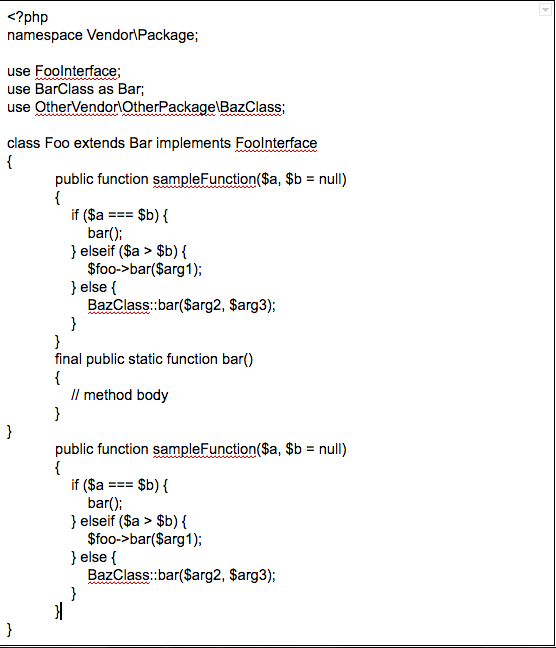
\includegraphics[width=1\textwidth]{images/ejemploCodigo1}
		\caption{Ejemplo de código}
	\end{figure}

% - - - - - - - - - - - - - - - - - - - - - - - - -
\subsection{Alternativas de solución}